\documentclass[10pt,a4paper]{article}

\usepackage{listings}
\usepackage{amsmath}
\usepackage{graphicx}
\usepackage{float}
\usepackage[hidelinks]{hyperref}
\usepackage[a4paper,left=3cm,right=3cm,top=2cm,bottom=2cm,bindingoffset=5mm]{geometry}

%opening
\title{Deep Reinforcement Learning Beginners Tutorial \\Documentation}
\author{Julian Bernhart, Robin Guth}

\begin{document}
	
	\maketitle
	\tableofcontents
	
	\section{Introduction}
	\textit{Deep Reinforcement Learning} is a huge step towards the creation of an universal artificial intelligence\footnote{can be used for multiple problems without notable changes}.
	In 2013 a company, owned by Google, called ''Deep Mind'', was able to create an astonishing implementation of RL\footnote{Reinforcement Learning}, which was capable to play a range of retro games of the console ''Atari 2600''.
	In many cases, the AI\footnote{Artificial Intelligence} was not only able to play the games successfully, but also exceeded human performances significantly \cite{atari}.
	After these impressive results, it is definitely worth to take a closer look at \textit{reinforcement learning}.\\	  
	Playing games is fun, but \textit{reinforcement learning} has more to offer, as discussed in \cite{usecasesRL}.
	Apart from playing video games, there are many use cases in fields like robotics, traffic control or even personalized advertisement.
	Apart from the Atari paper \cite{atari}, multiple papers have been written about RL.
	Some noteworthy examples are the creation of an RL algorithm, which recommends personalized news \cite{drn} or a survey about different applications for RL in robotics \cite{roboticsRL}. While supervised and unsupervised learning are already widely used in production, \textit{reinforcement learning} is still in development and further research is needed.
	As an interesting topic with many application possibilities, there is a demand for tutorials and hands-on guides for beginners, especially students.
	Beginners often struggle to find a good starting point into the world of AI and specifically RL.
	Many existing tutorials are written for more advanced users, who already have a deeper understanding of machine learning.\\
	For this reason, the \textit{''Deep Reinforcement Learning Beginners Tutorial''} was created, as an effort to create an easy to understand, hands-on guide to learn RL without needing extensive knowledge about \textit{machine learning}.
	After completing the tutorial, the reader will be familiar with the basics of RL and be able to create its own implementation based on the examples given.\\
	This document serves as a documentation of the making and thought-process of the authors, as well as a presentation of the result and a critical reflection of the work.
	First, the basic contents of the tutorial will be explained, to give the reader a short overview about the topic of RL.
	Then, the initial targets will be outlined as well as the methods and materials, that were used in the making.
	Finally, all results will be presented and evaluated against the initial targets. 
	This document will be concluded by the discussion of possible improvements and expansions of the final product.
		 
	%Section: Content//Deep Reinforcement Learning
	\section{Deep Reinforcement Learning}
	In this section we will discuss the content of two developed notebooks, mainly the theory behind Deep Reinforcement Learning (DRL). We will get to know the basic concept of RL, see on an exemplary neural network model the deep learning aspect and work out the necessary formulas in order to translate the theory into code. Further we will introduce a framework, which helps building this project by providing a game to play, more on that later.  All the theory, explanations and code can be viewed in completion in the enclosed notebooks:
	\begin{enumerate}
		\item Deep Reinforcement Learning Beginners Tutorial (1) - Theory 
		\item Deep Reinforcement Learning Beginners Tutorial (2) - Practice
	\end{enumerate}
	
motivation	

\subsection{The Software Agent}
	Befor we start with the topic of RL we have to adress some basics in order to clarify the following explaination. We will use the term of \textit{software agent}, which, as part of artificial intelligence, is a program, that acts self sufficient to solve a task. There are three important aspects an agent should fulfill. First are autonomous actions. An agent needs to make decisions without external help. Further an agent needs to execute multiple actions to complete its task, so it should be proactive. Last but not least, an agent has to be reactive, which means it reacts on changes in the environment it is in. An optional ability for an agent like this is independent improvement. For this the agent builds up knowledge after repetitively doing its task and improves itself this way.\\
	Basically, the part of the agent, which controls its actions, can be filled with different algorithms. In our case, this will be an implementation of RL, which fulfills all requirements of an agent.

\subsection{Reinforcement Learning}
	Reinforcement Learning is considered one of the three machine learning paradigms, alongside supervised learning and unsupervised learning. The main goal of RL is to create an agent, which can navigate by actions in an environment in a way to maximize a representation of a cumulative reward. The evironment is a space that contains the agent. We will talk about the environment later on. In order to miximize the reward, the agent has to learn by trial and error which actions most likely lead to a reward and which lead to a penalty. After some training, the agent will use its knowledge to avoid previous mistakes. It still has to explore the environment, because otherwise we can not be sure if we actually find the global maximum or just a local one and if there might be a better chain of actions. If we think about our real world, this method of learning is pretty close the human learning. If we get hurt for example, we are more likely to try to avoid the situation. Still curiosity or necessity leads us to exploring and thus maybe getting us into danger, but in the best case, will lead us to some kind of positive reward.\\
	
	\subsubsection{The concept of RL}
		Our agent is contained by an environment. A momentary snapshot of the environment is called state. A state contains all information at a certain point in time for example the position of the agent or enemies. There is a permanent exchange of information between the agent and its environment. The agent receives the actual state and has to choose an action based on its logic. Everything the agent can use to alter its environment is called an action. It changes the environment based on a certain set of rules. After executing an action the agents receives the new state and a reward, which helps to decide whether its decision leads to a positive result. Keep in mind, that a reward can also be negative. Basically, an environment is just a set of states. We can move between states by executing actions. A good example for an environment is our own world. We are agents, moving in the world. All the time we have to look at our surroundings and choose an action like moving accross the street or waiting until it is free. The laws of physics restrain us, take gravity for example. We receive rewards like geting hurt oder feeling satisfied, thats how we evalute our actions. Our environment is constantly changing, so we have to reevalute our decisions and choose an action again. The following picture shows the whole procedure:\\ 
% Bild einf�gen
		Our goal is to learn the best action for each state, so that our total reward reaches its global maximum.\\
		All components such as reward, amount and type of actions or states depend on the type of environment and can vary widely. As the real world example is pretty complex, for the rest of the notebook we will use a simple game environment for explanation. The informations available for an agent are the visual output of the game (actual state), the inputoptions and the reward for a previously taken action.\\
		The following diagram shows an exemplary setup for a RL project with a game as an environment. For the navigation through this environment the agent needs the actual state (game screen) as an input, in order to respond with an appropriate action. Every action taken leads to a value added to the score of the agent and a change in the environment resulting in the next state of the game.\\ 
		In order to improve its knowledge, the agent has to repeat the task multiple times. For this we define a set amount of epochs with a set amount of time for the agent to play.\\
		This is where the RL part comes into play. In order to maxmize the reward, the agent has to learn which actions result in a positiv reward and should be prefered and which ones should be avoided because of a penalty. In the beginning, the agent has no knowledge about the environment and thus cannot make an educated desicion. It will need to explore by taking random actions and observing the reward. These informations will be added to the knowledge of the agent. Over time the agent needs to decrease the amount of explorational actions and increase the amount of exploitational action in order to progress. This means that the agent will start to decide on an action based on its gained knowledge, while decreasing the amount of random actions. A good decreasing ratio is very important for RL, as changing to fast will lead to bad results, while changing it to slow will lead to overfitting.\\
		
	\subsubsection{Deep Learning Aspect}
		The agent has to recognize and differentiate elements in the environment, to be able to act accordingly and choose a proper action. In the best case, we already have the input reduced into some important numbers, which describe the actual state. In real applications this may not be possible or feasible with our knowledge. Most of the time we will have a picture available for example the image of a camera or a game screen, but the input we receive can basically be any sensory data.\\
		
		Furthermore the agent must associate the occurence of individual elements on screen with its own actions and the subsequent reward or penalty, which may occur only after several steps in the future. Depending on the situation it may be also necessary to estimate what the next state of the game could be. There are two possible ways to use the Deep Learning aspect.
		
		\begin{enumerate}
			\item Image processing with a Convolutional Neural Network (CNN), in order to process the image information and send this to the agent.
			\item A Deep Q-Learning Network (DQN), in order to model the Q-function, which is discussed below.
		\end{enumerate}
	
		Following is an exemplary presentation of a neural network, which is designed according to the tasks just mentioned.
		
% Bild einf�gen

		There are two ways to learn in deep reinforcement learning. Eiher we can use Value Learning or Policy Learning. With Value Learning, we assign values to each state-action pair, which correspond to the probabilities of the pair beeing the best option. In Policy Learning, we will learn a strategy instead, which gives as the best estimated action for a given state s. We will focus at Value Learning. 
			
	\subsubsection{Q-Learning}
		The task of the agent is the maximization of a cumulative future reward. An example of this can be the score in a game. In an environment, there is no guarantee for an immediate reward after executing an action. In many cases, only specific chains of actions lead to a positive reward, so the agent needs to learn multiple moves in succession in order to fulfill the given task. For example, if the agent needs to collect an object in order to get a higher score, it may be necessary to take multiple moves to reach it. The moves in between may not vary the reward significantly or even reduce it, however they are needed to complete the task in order to be successfull. 
		
		A simple way to implement RL is Q-Learning. We assign a numerical value to each action we can execute per state. This value is called Q-value. It represents an estimate of which action will result in the highest reward for the actual state. This is the knowledge of our agent. Each step we have to choose an action for the actual state. This is either random or knowledge based. We use random actions to explore our environment. If we use the knowledge of the agent, the next action is chosen by exploitation, so the agent uses the action with the highest Q-value for the given state. 
		
		The Q-Values are not known at the beginning and need to be learned by training. For this purpose, the agent needs to explore its environment. In the best case, it will visit all states through every possible action, but most of the time, this is neither needed nor possible, because of the amount of states or actions. We only desire the path with the best overall reward. We have to keep in mind, that there is no guarantee, that a path we found is the global maximum. It is possible, that the agent is stuck at a local maximum and needs to sacrifice some reward to be able to reach a state with a bigger payout. The Q-values are initialized by 0. After every step the agent takes, we need to update the last used Q-value according to the reward the agent receives. If the agent loses, dies or does something else we want to avoid, the resulting reward is negative. Either positive or negative, the Q-value needs to reflect this with its value. We need to update the Q-value regardless if the agent is exploring or exploiting. The exploration rate $\epsilon$ is slowly descending while training, so the agent can use its gained knowledge to improve the reward.
		
		In order to adjust the Q-values we need the total reward:
		
		$R_t = \sum\limits_{i=t}^{\infty} r_i = r_t + r_{t+1} + ... + r_{t+n} + ...$
		
		The \textit{total reward} $R_t$ is the sum of the actual reward and all future rewards from actual state \textit{t} to state  n = $\infty$.
		
		We also add a discount factor $\gamma$ to this formula. That factor has a range of value between/from $0$ to $1$ and is used to decrease rewards that are further into the future. This makes rewards in near future more dicisive for the agent. 
		
		$R_t = \sum\limits_{i=t}^{\infty} \gamma _i r_i = \gamma _{t} r_t + \gamma _{t+1} r_{t+1} + ... + \gamma _{t+n} r_{t+n} + ...$
		
		The total reward $R_t$ is the discounted sum of future rewards.
		
		After dicussing the Q-values our next step is the associated function. The Q-function is the name giving aspect of a Deep Q-Learning Network (DQN), while the "Q" stands for "Quality". The higher the reward, the higher the estimated Q-value and associated quality. This function represents the expected total future reward an agent could reach by executing a certain action $a_t$ in a given state $s_t$ and is used for our deep neural network. The DQN takes over the task of estimating this Q-value. With no prior information at the beginning, the agent needs to extends its knowledge by trial and error and thus learning, how to determine a Q-value out of the actual state and an action.
		
		$<$Q-Value depending on $s$ and $a$ $> = <$Expected total future reward$>$\\
		
		$Q(s, a) = E[R_t]$
	
		If we have a good approximation of the Q-values for each state-action-pair after the exploration, the agent needs to decide on which action is the best for a given state. This means the agents needs to choose the action which maximizes the estimated future reward by the associated Q-value, with the help of a policy $\pi^*(s)$. This is the part of exploiting the gained knowledge.
		
		$<$Optimal policy depending on $s$$> = <$Action resulting in the highest future reward according to current knowledge$>$

		$\pi^*(s) = {\underset{a}{\operatorname{argmax}}Q(s,a)}$
		
		Finally, we will take a look at the formula, which we will actually use to calculate Q-values. At the moment we use the current state of the environment, the actions to take and the reward, resulting from the decision of the agent as input. We also use the following state of the environment. We introduce the \textit{Bellman equation}  now:
		
		$<$Q-value depending on $s_t$ and $a_t$ $> = <$ Reward observed after the last action (immediate reward)$> + <$ Discount factor $> * <$ Maximum Q-value for the next state of the game (future reward)$>$

		$Q(s_t, a_t) = r_t + \gamma * \max\limits_{a'} Q(s', a')$
		
		For now the Bellman equation provides the Q-value for a given action in a given state. In order to train our DQN regarding the Q-function, it is necessary to compare the Q-values predicted with the actual ones and minimize the error between the two. If we use the Bellman equation to calculate this difference, by simply subtracting these values, we get the so called \textit{temporal difference error}.
		
		$<$Temporal difference error$> = <$ Target Q-value$> - <$ Predicted Q-value$>$

		$\delta = ( r_t + \gamma * \max\limits_{a'} Q(s', a')) - Q(s_t, a_t)$
		
		To update an old Q-value, we use the temporal difference error and add it to the Q-value. A new discount factor, called learning rate $\alpha$, determines the weight of the temporal difference error.
		
		$<$new Q-value depending on $s_t$ and $a_t$ $> = <$old Q-value depending on $s_t$ and $a_t$ $> + <$Temporal difference error$>$

		$Q(s_t, a_t)_{new} = Q(s_t, a_t)_{old} + \alpha * \delta$
		
		Now we use \textit{gradient descent}, an optimization algorithm, to optimize the Q-value approximation. Therefor we can train the DQN using \textit{mean square error} as the loss function, which results in the the following formula.
		
		$L = E[\lVert \delta \rVert ^2]$
	
	\subsubsection{Model Q-function}
		The following illustration shows two options by which we can model our Q-function with a deep neural network. The model on the left side estimates one Q-value at the time. This is what we are using at the moment. The model on the right side is the prefered one, because it increases the efficiency. It gets the state of the environment and calculates multiple Q-values, so we just have to choose the highest value to determine the action for the agent instead of estimating the Q-values for every action individually. This will save processing power, as the amount of possible actions can be very large.
		
%Bild einf�gen

\subsection{The OpenAi Gym Framework}
	

\subsection{The Exercises}
	
	


	\section{Initial Targets}
		As the reader is now familiar with the topic of RL, in this section, the initial targets will be discussed. Later on, these targets are critically compared to the results. Some of the presented targets may overlap.
		
		\begin{description}
			\item[Beginner-Friendly] 	The main goal in the creation of this tutorial is to create an easy understandable, hands-on beginners guide to RL.
			This means that there need to be extra steps to reach this target like:
			\begin{itemize}
				\item extensive, comprehensive explanations
				\item explanations for new terms
				\item accompanying images/visualizations
				\item easy language
				\item explained code examples
				\item simple exercises with solutions
				\item inviting environment 
				\item no big obstacles without support
				\item easy to set up
				\item etc.
			\end{itemize}
			
			\item[Topic] The focus should be on the basics of RL, as well as everything the reader needs to be able to understand and write its own agents. There should be a theory part as well as accompanying code examples.
		
			\item[Relevant Knowledge] After the completion of the tutorial, the user should be able to proceed with other tutorials or sources, without needing to start over again. The knowledge presented should contain necessary and useful basics of RL.
			
			\item[Easy Code] As the target for the tutorial is to teach the reader how to use RL, there need to be some code examples. For this an easy programming language is needed, which is relevant for RL and not just used for examples. The code should also be commented and explained.\\ 
			
			\item[Combination of text and code] Many tutorials in existence require the installation of additional software, like compilers for the programming language. This separates the code from the theory and explanations. For this reason, the code and text should be in the same document, so that a reader can instantly run code while reading the explanations. 
			
			\item[Performance] An important point to consider is the required computing power to train an agent. As many thousands to millions of steps are needed, this is more than most personal computers can handle in a decent amount of time.  
			For this reason, the tutorial should be based on the usage of a cloud service to execute code. 
			This delivers enough computational power to train an agent in a short period of time, as well as separating the execution environment from the users personal hardware, which removes the need to install software on the users pc.
			
			\item[Budget-Friendly \& Accessible] As this tutorial is aimed at beginners, who may just want to take a quick look at RL, it is important that the tutorial can be used without obstacles. For this reason, the tutorial should be freely available, as well as usable without costs or very low cost.
		\end{description}

	\section{Methods and Materials}
		In this section, the methods and materials used in the creation of the tutorial are presented, as well as the thought process of the authors.

		\subsection{Python} As the programming language \textit{Python} is dominating fields like \textit{data science} or \textit{machine learning}, was made with the intention of creating a very simple programming language and many libraries being written in \textit{Python}, this seems an excellent choice for this tutorial.\\ 

		\subsection{Jupyter Lab}
		\textit{Jupyter Lab} was chosen as an environment to develop and execute Python code, as well as the place to combine explanations, pictures and code into one document.\\
		It is basically an editor for jupyter notebooks.
		A notebook is a document with multiple successive cells, which can be one of the following types. 	\begin{description}
			\item[Code] A cell filled with \textit{Python} code.
			\item[Markdown] A cell filled with \textit{Markdown} instructions.
			\item[Raw] A cell with raw data representation, is not used generally.
		\end{description} 
		The Lab provides support for the typesetting language ''Markdown'', which enables the authors to create stylized text sections with images and other features like table of content, web links etc.
		Each cell can be executed individually, to either create console output or stylized text, so a reader can be guided step by step.
		A section of an exemplary notebook is shown in image \ref{jupLab}.\\
			\begin{figure}[h!]
			\begin{center}
				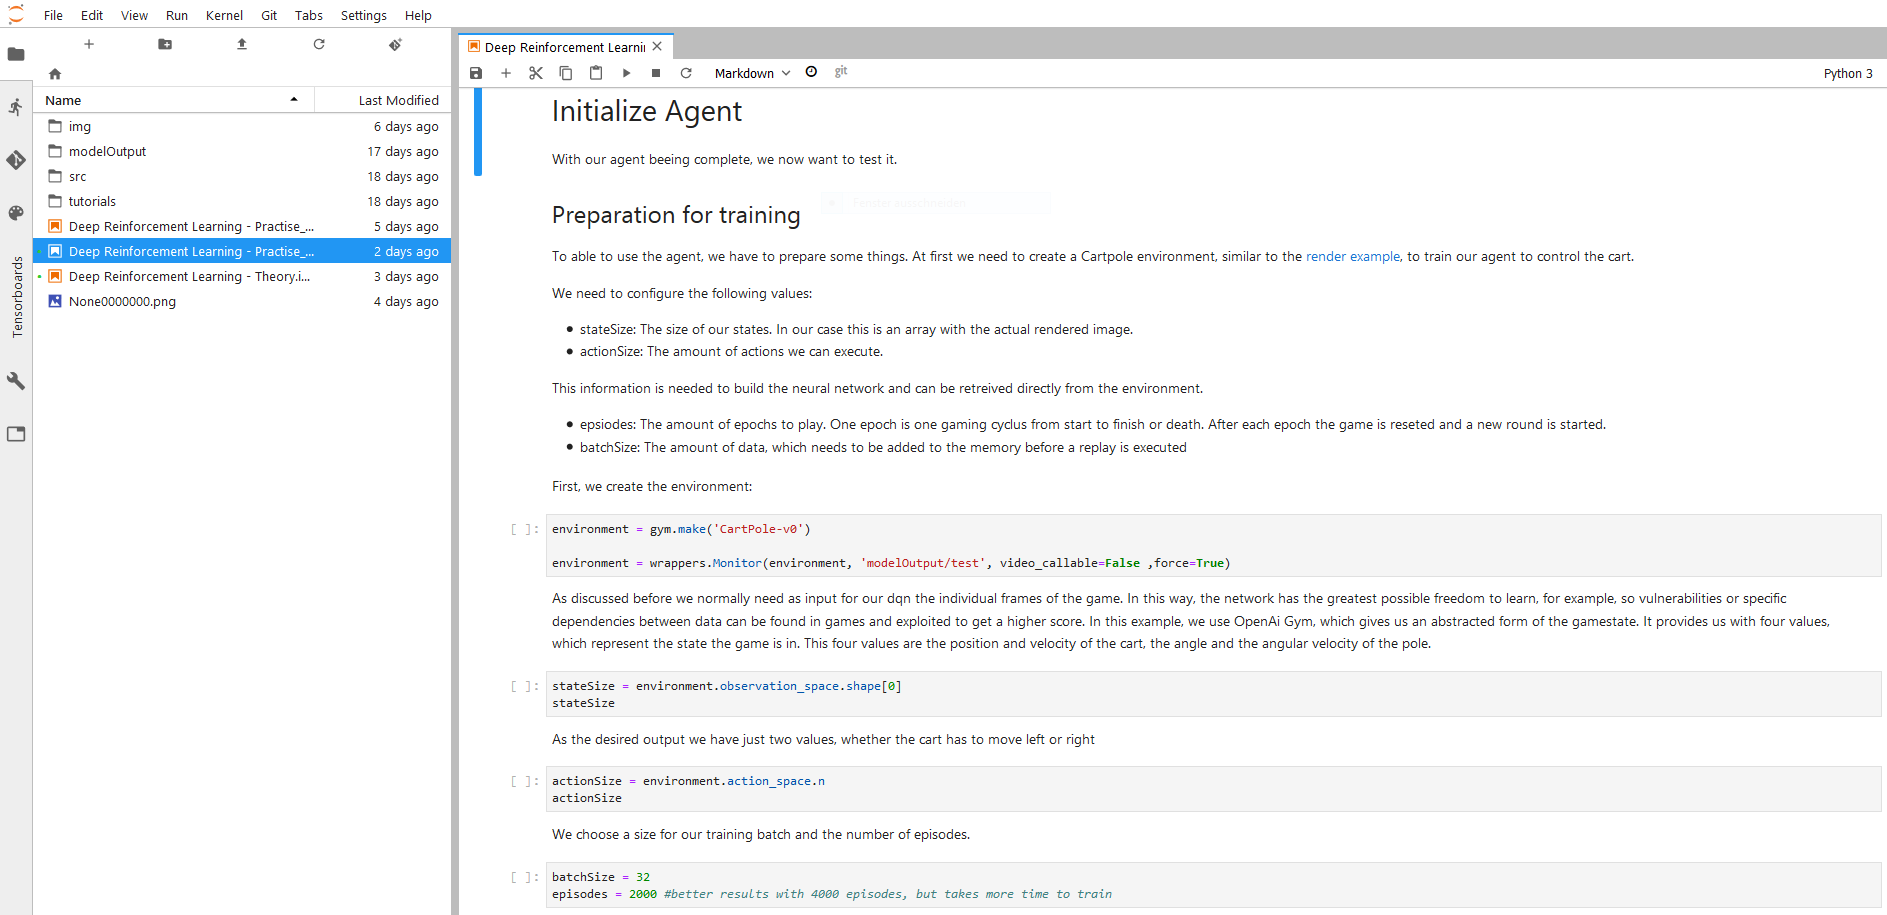
\includegraphics[width=\linewidth]{img/jupLab.png}
				\caption{Jupyter Lab}
				\label{jupLab}
			\end{center}
		\end{figure}
		The usage of \textit{Jupyter Lab} has many advantages like:
		\begin{description}
			\item [Unified environment] Every user has the same development environment. This reduces the probability of errors and simplifies the installation process.
			\item[Easy-to-use] Jupyter Lab provides an easy to use interface.
			\item[Code integration] The cell based notebooks include executable code. There is no need to copy code and the code can be placed after corresponding explanations.
			\item[Easy dependeny installation] Jupyter Lab supports the installation of Python libraries through simple commands.
		\end{description}
		Further information on Juypter Lab and its notebooks can be found at \url{https://jupyterlab.readthedocs.io/en/stable/}.
		
		\subsection{Libraries}
		As it is common in programming, third-party libraries provide prewritten code, so that a user does not have to implement basic tasks on its own.
		The following libraries are used in the notebooks:
		\begin{description}
			\item[NumPy] Scientific computation in Python (n-dimensional arrays).
			\item[Tensorflow] Open source machine learning library.
			\item[Keras \& KerasRL] High level implementations of neural networks and different RL algorithms. 
			\item[OpenAI Gym] Provides different machine learning environments based on games.
		\end{description}
		
		\noindent As OpenAI Gym is quite relevant in the world of AI, it is discussed in greater detail. The other libraries are quite common and provide basic utilities, there is no need to discuss them further. 
		
		\subsubsection{OpenAI Gym}
		Developing \textit{machine learning} algorithms is often neither easy to understand nor comprehensible especially for beginners.
		As most people are familiar with video games, game are simple and completely observable environments.
		OpenAI Gym is an open source framework, which delivers a range of different game environments. It provides all environmental data an RL agent needs and using an existing game makes it also easier to compare the agent to human performance or other agents and therefore the evaluation of different algorithms is easier.
		Another advantage is, that a developer does not need to build a dedicated testing environment and saves time.
		
		\subsection{Google Cloud}
		As discussed before, a normal personal computer is to slow to train an agent in a decent amount of time. For this reason, a cloud based approach is chosen.\\
		The cloud service of Google, \textit{Google Cloud}, provides an already preconfigured virtual machine based on the operating system \textit{Linux}.
		With this, Jupyter Lab can be run on a server with more processing power and the installation process is easier, because the user just has to choose the vm\footnote{Virtual Machine} template and it will be automatically installed. 
		This also eliminates the need for the user to install software on the users personal machine and makes it possible to use lower-end machines like laptops to access the vm online. 
		With these advantages, there is also one main disadvantage: As a service of Google, the use of the vm costs money. 
		Luckily, Google offers free credit for students after registration.
		If this is no option for an user, the use of a cloud is fully optional and the environment of Jupyter Lab can be installed locally without any problems. 
		In terms of ease-of-use, the cloud service is a good choice.
		
		\subsection{Source Materials}
		As RL is a fairly new topic, changes may still occur. For this reason, the used source materials are mostly available online.\\
		The base for the theory part is a freely available lecture\footnote{Lecture of MIT: \url{https://www.youtube.com/watch?v=i6Mi2_QM3rA}} of the MIT.\\
		The code is based on a video series about RL\footnote{Deep Q Learning Networks: \url{https://www.youtube.com/watch?v=OYhFoMySoVs}}.  
	
	\section{Results}
	 
	 In this section, the final result of the efforts to create a deep reinforcement learning tutorial is presented. 
	 First, the produced notebooks and other documents are discussed in depth.
	 Then, these results will be compared against the initially set targets.
	 
		\subsection{Products}
		The following documents were created in the making of the tutorial:
		\begin{itemize}
			\item Notebook1 - Theory behind RL.
			\item Notebook2 - Practical example with OpenAI Gym.
			\item Installation Guide
			\item Documentation
			\item Poster about the Documentation
		\end{itemize}
		\subsubsection{Notebooks}
		
			\paragraph{Notebook 1 - Theory}
				This notebook, is mainly used to explain the basics of RL to the reader.
				In the beginning, the concept of software agents is explained as well as the basic concept of RL.
				The usage of neural networks in RL is discussed.
				Two types of reinforcement learning are introduced: \textit{value learning} and \textit{policy learning}.
				One example for \textit{value learning} is explained in depth, the so called \textit{Q-learning}. 
				The main formula for Q-learning is derived out of simpler formulas.
				Finally, an outlook is given, mainly about the second notebook.
			\paragraph{Notebook 2 - Practice}
				In the second part of the tutorial, the reader can finally start to program an agent. 
				Before that, OpenAI Gym and the chosen environment is introduced.
				Also, the rendering of the training process is explained.
				The main part of this notebook is the creation of a fully functional RL agent step-by-step.
				The tutorial is concluded by an reflection on the things the reader learned and an outlook into further readings and tutorials.
			\subparagraph{Exercises}
			The exercises are a comparatively small part of the notebooks. The main goal is to explain \textit{deep reinforcement learning}. The notebooks were designed to be easily understandable with a good connection between theory and implementation. All code passages are explained in detail, so that the project can be comprehended in its entirety. The goal of the exercises is to build and understand a basic structure for a RL agent. The individual tasks are located at the points in the code where the agent can be further optimized and customized to create an entry point into a project.
		\subsubsection{Ease of Use}
		A very important target while developing the notebooks was to keep the tutorial easy-understandable and usable, as well as having a tutorial with an useful amount of information. In this section, some steps are presented, which were taken to increase the ease of use.
			\paragraph{Installation Guide}
			After Google Cloud and Jupyter Lab became central parts of the experience, it became clear, that a potential user may not have the needed knowledge to set up the environment. A full installation guide was created, which guides the user through the installation process with the \textit{Google Cloud}.
			\paragraph{Usage of ''We''}
			A tutorial should always be welcoming and invite the reader to explore the topic without to big obstacles in the way. For this reason, the notebooks are both using ''we'' as a way to make the user feel like he is not alone, even if there is frustration, while trying to understand the concepts.\\
			Example: ''Before we head into the world of reinforcement learning, we will have to talk about software agents.'' - out of notebook 1
			\paragraph{Visualization}
			Another important goal is to make the training epochs visible. This was not easy to achieve with the cloud and Jupyter Lab, but the final result lets the user create a gif out of a training episode, which can be viewed after the training. The following picture \ref{cartpole} shows a part of an created gif:
			
			\begin{figure}[h!]
				\begin{center}
					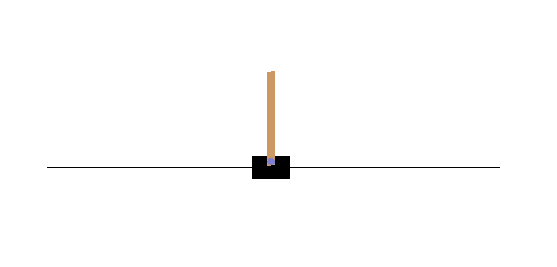
\includegraphics[width=0.6\linewidth]{img/cartpole01.png}
					\caption{Visualizing the training}
					\label{cartpole}
				\end{center}
			\end{figure}
		
		\subsubsection{Cartpole}
			The game Cartpole was chosen as the environment for the agent. The goal of Cartpole is to balance a pole on a cart, which can move to the right or left. If the pole tips over the game is lost. This game is an excellent choice for an environment, as its a really simple game, which is great for explaining things without distracting to much.
			In image \ref{cartpole} a round of Cartpole can be seen.
			
	\subsection{Initial Targets vs. Result}
	
		In this section, the initial targets are compared against the final results.
		
		\begin{description}
		\item[Beginner-Friendly] The final product are two notebooks and the installation guide. The theory as well as the practice are explained and code is commented. 
		Comprehensibility is a subjective opinion, but many steps were taken to assure an easy understandable tutorial.
		The text is accompanied by images, to illustrate explanations.
		There are many code examples and exercises written in Python.
		Finally, there is an extensive installation guide to install the whole tutorial.
		
		\item[Topic] The initial topic was fulfilled in the final product with two notebooks, one dedicated to theory and one to practice. 
		
		\item[Relevant Knowledge] As discussed, the basics of RL are explained in the first notebook.  
		
		\item[Easy Code] As the target for the tutorial is to teach the reader how to use RL, there need to be some code examples. For this an easy programming language is needed, which is relevant for RL and not just used for examples. The code should also be commented and explained.\\ 
		
		\item[Combination of text and code] With the usage of Jupyter Lab, code and text are successfully combined into one document. 
		
		\item[Performance] The usage of Google Cloud enables the reader to use a fully powered server to execute the agent. This target was also fulfilled.
		
		\item[Budget-Friendly \& Accessible] With the increased performance, which is reached by using Google Cloud as a server provider, the tutorial may cost a user small amounts of money, if the tutorial is run in the cloud. 
		But as the tutorial can also be executed locally on a personal computer, this is not much of a constrain. 
		If a user really wants to dive into the world of RL anyway, powerful hardware is needed, so this is more of a constraint of RL in general then of this tutorial.
	\end{description}
	\subsection{Further Improvements}
	In this section, problems with the result are discussed and solutions are offered.
	
	\subsubsection{Policy Learning}
		The notebooks only cover value learning, this should be extended to also include policy learning, as this is a more advanced technology to train an agent. 
		This would improve both notebooks. 
		In notebook 1, policy learning would be introduced and explained.
		Theoretical advantages and disadvantages would be discussed.
		In the second notebook, there would be another version of the implemented agent, that would be using an implementation of policy learning.
		Finally both agents would be compared and evaluated.
		
	\subsubsection{More exercises}
		At the moment, there are only three exercises for the reader to complete. In the future, there should be more exercises to help with the understanding as well as extending the knowledge of the reader.
		
	\subsubsection{More code \& libary explanation}
		Another useful extensions of the tutorial would be to show more code and explain a library, which already implemented algorithms like DQN.
		
	\subsection{Conclusion}
	
	The authors were able to create a beginners tutorial, which will hopefully help many people to make their first steps into the exiting world of \textit{deep reinforcement learning}.
	\bibliography{bib} 
	\bibliographystyle{ieeetr}
\end{document}
